%% Paper B: paired SHAP-LIME comparison. CLEI Electronic Journal edition
%% (single-blind; cleiej.cls from the journal, unmodified).
%%
%% Reduced on 2026-10-04 from the 32-page paper_bc_iberamia.tex (ADR-0022).
%% No result was changed: every number is registered in
%% pub/claim_registry.toml. The taxonomy, the scoping corpus and the
%% LLM-judge study are not in this paper.
\documentclass{cleiej}
\usepackage{amssymb}
\usepackage{amsmath}
\usepackage{graphicx}
\usepackage{booktabs}
\usepackage{tabularx}
\usepackage{array}
\usepackage{enumitem}
\usepackage{url}
\usepackage[hidelinks]{hyperref}
\setlength{\emergencystretch}{3em}
\setlist{nosep,leftmargin=*}

% Version DOI of the Zenodo release that archives exactly this study.
\newcommand{\zenodoversiondoi}{\url{https://doi.org/10.5281/zenodo.23147228}}

% Double-blind build: paper_b_cleiej_blind.tex defines \blindreview and then
% inputs this file. It hides the author block, the acknowledgments, the
% repository address and the archive DOI. The journal itself reviews
% single-blind; the default build is the one to submit there.
\newif\ifblind
\ifdefined\blindreview\blindtrue\fi

\title{When Does SHAP Outperform LIME? Model- and Configuration-Dependent
Results from a Paired Tabular Benchmark}

\ifblind
\author{\it Authors omitted for double-blind review}
\else
\author{
\bf Jonathan Herrera-V\'asquez\\
Universidad Americana de Europa (UNADE), Department of Computer Science,\\
Canc\'un, Quintana Roo, Mexico,\\
\it jonnabio@gmail.com
}
\fi

\begin{document}
\maketitle

\begin{abstract}
\noindent
% AUTO-GENERATED FILE. Source: pub/claims.toml
LIME and SHAP are the most widely used model-agnostic explainers for tabular
models, yet controlled paired comparisons of the two remain scarce. This
paper extends an earlier paired test to the full grid of a public benchmark:
75 cells that share model, seed and sample size, over five model families on
the UCI Adult census-income dataset, with Holm-corrected paired tests and
effect sizes for five endpoints. SHAP leads on stability ($d_z{=}3.00$),
fidelity ($d_z{=}4.82$) and faithfulness gap ($d_z{=}2.63$), and LIME gives
sparser explanations. Two results depend on conditions that are usually left
implicit. First, the latency ordering depends on the model family: SHAP's
\texttt{TreeExplainer} was faster than LIME in every XGBoost cell and slower
in every random-forest cell, and LIME was faster for non-tree models (median
53.3 ms vs.\ 694.6 ms). Second, LIME's near-zero stability on Adult is not a
fixed property of the method: it is high on two further tabular datasets
and, in a single-model probe, rises with the kernel width. The results support choosing the explainer
according to the model architecture and the latency budget, and they show
that a ranking obtained on one dataset and one configuration does not
transfer by default. All artifacts are public.

\end{abstract}

\keywords{% AUTO-GENERATED FILE. Source: pub/claims.toml
explainable artificial intelligence, LIME, SHAP, explanation evaluation, benchmarking
\unskip.}

% -----------------------------------------------------------------------
\section{Introduction}
\label{sec:intro}
% -----------------------------------------------------------------------

LIME~\cite{ribeiro2016why} and SHAP~\cite{lundberg2017unified} are the two
most widely used model-agnostic post-hoc explainers for tabular models. A
practitioner who must choose one of them needs to know how they differ in
the properties that matter for the deployment: whether an explanation tracks
the model, whether it is stable, how many features it uses and how long it
takes. Their theoretical differences are well known, but they do not by
themselves settle the choice across model families, sampling regimes and
runtime constraints~\cite{retzlaff2024posthoc,ali2023trustworthy}.

The empirical guidance is weaker than the popularity of the two methods
suggests. Evaluation of explanations is spread over several metric
families, and comparisons between explainers often depend as much on the
metric chosen as on the methods
themselves~\cite{nauta2023anecdotal,canha2025benchmark,longo2024manifesto}.
Work that uses several metrics shows that fidelity, stability, sparsity and
cost carry complementary
signals~\cite{pawlicki2024metrics,zheng2025ffidelity}. Controlled
comparisons of LIME and SHAP under matched conditions, where the two
explainers see the same model, the same instances and the same random seed,
remain scarce. Without that pairing, a difference between the methods cannot
be separated from a difference between the models or the samples they were
run on.

This paper reports such a paired comparison. It reuses the execution cohort
released with an earlier study~\cite{herrera2026framework}, which introduced
the measurement protocol and compared four explainer families. That study
already contains a first paired test of SHAP against LIME, on the 45 matched
cells of three model families (logistic regression, random forest and
XGBoost): SHAP was higher on fidelity, stability and faithfulness gap, and
LIME was cheaper and sparser. It announced the analysis on the full grid of
75 cells without reporting it, and it reported averages over conditions
only. The present paper completes that contrast on the 75 cells of the five
model families, with confidence intervals and effect sizes, and then asks
the question that an average over conditions hides: \emph{when does the
answer depend on the model and on the configuration?}

The paper makes three contributions:
\begin{enumerate}
\item \textbf{Paired inferential evidence on the full grid.} The SHAP--LIME
difference, tested before on a 45-cell subset, is quantified on the 75
matched cells of the UCI Adult census-income dataset, over five model
families, with Holm-corrected paired tests, confidence intervals and effect
sizes for five endpoints (Section~\ref{sec:results}).
\item \textbf{Two conditional results.} The latency ordering of the two
methods depends on the model family, and reverses between two tree
ensembles (Section~\ref{sec:runtime}). LIME's near-zero stability on Adult
depends on the kernel width and on the feature space, and is high on two
further datasets (Sections~\ref{sec:exp3} and~\ref{sec:kernel}).
\item \textbf{A deployment recommendation conditioned on the model
architecture}, with an explicit statement of which claims generalize and
which do not (Section~\ref{sec:discussion}).
\end{enumerate}

The paper makes ranking claims under a stated protocol. It does not claim
that either method is correct for a task, and it does not test whether users
decide better with either explainer.

% -----------------------------------------------------------------------
\section{Background and Related Work}
\label{sec:background}
% -----------------------------------------------------------------------

\subsection{LIME}

LIME approximates a black-box model $f$ locally around an instance $x$ by
training an interpretable surrogate $g$ on perturbed samples weighted by a
kernel $\pi_x$:
\begin{equation}
\xi(x) = \arg\min_{g \in G} \mathcal{L}(f, g, \pi_x) + \Omega(g),
\label{eq:lime}
\end{equation}
where $\xi(x)$ is the explanation returned for $x$, $G$ is the class of
interpretable surrogates (sparse linear models here), $\mathcal{L}$
measures how poorly $g$ reproduces $f$ on perturbed samples, each sample
weighted by its proximity $\pi_x$ to $x$, and $\Omega(g)$ penalizes
surrogate complexity~\cite{ribeiro2016why}. LIME's behavior is shaped by
the hyperparameters that build the neighborhood: the kernel width, the
number of perturbed samples and the feature budget. These controls yield
compact explanations and low latency, but they introduce stochastic
variation, because local neighborhoods are sampled rather than exhaustively
enumerated.

\subsection{SHAP}

SHAP explains a prediction through additive feature attributions
$f(x) = \phi_0 + \sum_{i=1}^{M} \phi_i$, where $\phi_0$ is the model's
expected output over a background sample, $M$ is the number of features and
$\phi_i$ is the Shapley-value contribution of feature $i$. SHAP values are
the unique additive attributions that satisfy local accuracy, missingness
and consistency~\cite{lundberg2017unified}. KernelSHAP estimates them with
a weighted regression over feature coalitions and applies to any model;
tree-specific implementations exploit the model structure for speed.
Relative to local-surrogate methods, SHAP is typically denser and, outside
tree models, computationally heavier, because many coalition evaluations
are required.

\subsection{Evaluating and Comparing Explainers}

Quantitative evaluation of explanations relies mostly on proxy metrics that
need no human judgment: fidelity or faithfulness under feature
removal~\cite{bhatt2020evaluating,samek2017evaluating,hooker2019benchmark},
robustness of the explanation to small changes of the
input~\cite{alvarezmelis2018robustness}, and structural properties such as
sparsity. Toolkits and benchmarks standardize these
measurements~\cite{hedstrom2023quantus,agarwal2022openxai}, and systematic
reviews document how unevenly they are
applied~\cite{nauta2023anecdotal,canha2025benchmark}. Several results warn
against reading a proxy score as correctness: attribution methods can pass
perturbation tests and fail sanity checks~\cite{adebayo2018sanity},
removal-based scores depend on the removal
scheme~\cite{rong2022consistent}, and LIME and SHAP can both be
manipulated~\cite{slack2020fooling}. Shapley-value attributions have known
limitations as importance measures when features are
dependent~\cite{kumar2020problems}.

For a fair comparison of LIME and SHAP, confounders unrelated to the
explainer must be controlled. This motivates the protocol of
Section~\ref{sec:methods}: an identical transformed feature space, shared
model artifacts, a fixed class target, and cells matched on
$(\mathrm{model}, \mathrm{seed}, N)$. Under these controls the expected
trade-offs become testable: LIME should favor sparsity and speed, and SHAP
should favor stability and faithfulness.

% -----------------------------------------------------------------------
\section{Materials and Methods}
\label{sec:methods}
% -----------------------------------------------------------------------

\subsection{Cohort and Research Questions}
\label{sec:rqs}

The runs analysed here come from the execution cohort released by
Herrera-V\'asquez and Herrero-Uceda~\cite{herrera2026framework}, under the
protocol and reproducibility contract defined there. The analysis is not
the same: that study reports an omnibus comparison across four explainer
families at the block level and a paired SHAP--LIME test restricted to 45
cells of three model families. The present analysis covers the 75 matched
cells of the five families at the run level, with directional hypotheses,
Holm-corrected paired tests, confidence intervals and per-endpoint effect
sizes, and it examines how the differences vary with the model family, the
dataset and the LIME configuration. Reusing the cohort is deliberate: a fresh
execution would add environment variation to a comparison whose purpose is
to isolate the explainer.

Four directional questions are addressed, each with its hypothesis, where
$S$ is stability, $P$ sparsity, $C$ cost and $F$ fidelity:
\begin{itemize}
\item \textbf{RQ1 (robustness).} Is SHAP more stable than LIME under input
perturbation? $H_1: S_{\mathrm{SHAP}} > S_{\mathrm{LIME}}$.
\item \textbf{RQ2 (parsimony).} Is LIME sparser than SHAP?
$H_2: P_{\mathrm{LIME}} < P_{\mathrm{SHAP}}$, where $P$ is the
active-feature ratio (lower is sparser).
\item \textbf{RQ3 (efficiency).} Is LIME computationally cheaper than SHAP?
$H_3: C_{\mathrm{LIME}} < C_{\mathrm{SHAP}}$.
\item \textbf{RQ4 (faithfulness).} Does SHAP give stronger fidelity and
faithfulness signals than LIME? $H_4: F_{\mathrm{SHAP}} > F_{\mathrm{LIME}}$.
\end{itemize}

\subsection{Experimental Design and Analysis Units}
\label{sec:design}

The benchmark has four factors: model family
$g \in \{\mathrm{logreg}, \mathrm{rf}, \mathrm{xgb}, \mathrm{svm},
\mathrm{mlp}\}$; explainer $k \in \{\mathrm{LIME}, \mathrm{SHAP}\}$; seed
$s \in \{42, 123, 456, 789, 999\}$; and sampling intensity
$N \in \{50, 100, 200\}$ instances per stratum of the confusion matrix
(TP, TN, FP, FN). This yields $5 \times 2 \times 5 \times 3 = 150$ planned
runs, all of which are artifact-qualified (75 LIME, 75 SHAP), forming 75
matched SHAP--LIME cells on identical $(g, s, N)$ coordinates.

To avoid pseudoreplication, the analysis is hierarchical: metric values are
computed per instance, averaged per run, and the paired SHAP--LIME run
means on shared $(g, s, N)$ cells are the inferential unit.

\subsection{Data, Models and Explainer Protocol}
\label{sec:data}

All experiments of the main cohort use the UCI Adult
dataset~\cite{kohavi1996scaling,becker1996adult} with a stratified split
and deterministic seeds. The preprocessing pipeline is fitted on the
training partition only, with numeric scaling and one-hot encoding of
categorical features, which gives 103 transformed features. A fixed set of
pre-trained models is shared across all explainer runs to isolate the
explainer effect: random forest~\cite{breiman2001random}, gradient-boosted
trees~\cite{chen2016xgboost}, logistic regression, a support vector machine
(SVM) and a multilayer perceptron (MLP). Evaluation instances are sampled
by confusion-matrix stratum. Realized instance counts range from 27 to 800
(median 400).

Both explainers consume the same transformed feature space and target the
probability of the positive class:
\begin{itemize}
\item \textbf{SHAP:} \texttt{TreeExplainer} for tree models and
\texttt{KernelExplainer} for the other models, with a background sample of
$n=50$.
\item \textbf{LIME:} tabular local surrogate with a feature budget of
\texttt{num\_features=10}, an effective \texttt{num\_samples=1000} and
\texttt{kernel\_width=3.0}.
\end{itemize}
\label{sec:explainer_protocol}
These are fixed reference settings, not the library defaults. The
sensitivity of the results to the LIME kernel width is examined in
Section~\ref{sec:kernel}.

\subsection{Metrics}
\label{sec:metrics}

The metrics follow the protocol of the earlier
study~\cite{herrera2026framework}. Throughout, $f(x)$ is the model's
predicted probability of the positive class, $e(x) \in \mathbb{R}^{M}$ is
the attribution vector an explainer returns for instance $x$ with $M$
features, and ``masking'' feature $j$ replaces its value with the
training-set mean $\bar{x}_j$.
\begin{enumerate}
\item \textbf{Stability} $S$: robustness of the explanation to small input
noise~\cite{alvarezmelis2018robustness}. The explainer is run on $T=15$
perturbed copies $x^{(a)} = x + \varepsilon^{(a)}$, with
$\varepsilon^{(a)} \sim \mathcal{N}(0, \sigma^2 I)$ and $\sigma=0.1$,
and $S$ is the mean cosine similarity over all $T(T-1)/2$ pairs of
the resulting attribution vectors $e^{(a)} = e(x^{(a)})$:
\begin{equation}
S = \frac{2}{T(T-1)}\sum_{1 \le a<b \le T}\cos\!\left(e^{(a)},e^{(b)}\right).
\label{eq:stability}
\end{equation}
$S$ is $1$ when every perturbation yields an attribution vector with the
same direction, and near $0$ when directions are unrelated.
\item \textbf{Sparsity} $P$: active-feature ratio, the share of the $M$
features whose absolute attribution exceeds the threshold $10^{-4}$. A
lower active ratio means a sparser explanation.
\item \textbf{Fidelity} $F$: a single-feature variant of the faithfulness
correlation of Bhatt et al.~\cite{bhatt2020evaluating}. Each feature $j$ is
masked on its own, giving the masked instance $\tilde{x}^{(j)}$, and
\begin{equation}
F = \rho\!\left(\bigl\{|e_j(x)|\bigr\}_{j=1}^{M},\;
\bigl\{|f(x) - f(\tilde{x}^{(j)})|\bigr\}_{j=1}^{M}\right),
\label{eq:fidelity}
\end{equation}
where $\rho$ is the Pearson correlation across the $M$ features. $F$ is
high when the features an explanation ranks as important are those whose
removal moves the prediction most.
\item \textbf{Faithfulness gap} $\Delta_k$: a deletion test in the spirit
of~\cite{samek2017evaluating,hooker2019benchmark}. The $k=5$ features with
the largest $|e_j(x)|$ are masked together, giving
$\tilde{x}^{(\mathrm{top}\text{-}k)}$, and
\begin{equation}
\Delta_k = \left|f(x) - f\!\left(\tilde{x}^{(\mathrm{top}\text{-}k)}\right)\right|.
\label{eq:gap}
\end{equation}
A larger $\Delta_k$ means the features the explanation names first carry
more of the prediction.
\item \textbf{Cost} $C$: per-instance wall-clock explanation time (ms).
\end{enumerate}

LIME's active-feature count is bounded by \texttt{num\_features=10}, which
is a hard ceiling on the number of non-zero attributions. LIME's sparsity
is therefore a consequence of a hyperparameter, not an emergent property of
the method. The active-feature ratio measures whether LIME, \emph{as
configured}, returns fewer significant features than SHAP; it does not test
whether LIME is intrinsically sparser.

\subsection{Inferential Protocol}
\label{sec:inference}

The statistical plan follows established practice for comparing learning
methods~\cite{demsar2006statistical}: a two-sided paired Wilcoxon
signed-rank test on the matched cells for each
metric~\cite{wilcoxon1945individual}; the paired effect size $d_z$ for
magnitude~\cite{lakens2013calculating}; and Holm--Bonferroni control of
multiplicity over the five primary metrics~\cite{holm1979simple}. All
inferential claims are restricted to artifact-qualified runs: parseable,
non-empty results with explicit matched pairing.

\subsection{Reproducibility and Computing Infrastructure}
\label{sec:infrastructure}

The protocol is configuration-driven (YAML files with seeded execution).
Each run writes a \texttt{results.json} artifact; malformed or empty runs
are excluded explicitly and nothing is imputed. All experiments ran on CPU.
The reference software environment is Python~3.11 with scikit-learn~1.7.1,
XGBoost~3.1.2, SHAP~0.50.0, LIME~0.2.0.1, NumPy~2.2.6, pandas~2.3.3 and
SciPy~1.16.3, pinned in the repository. Runs were executed on several
commodity workstations under macOS, Windows and Linux, distributed by a
work queue. Each run artifact records its configuration, seed, timestamps
and duration; processor and memory specifications were not recorded. The
consequence for the cost endpoint is discussed in
Section~\ref{sec:validity}.

% -----------------------------------------------------------------------
\section{Results}
\label{sec:results}
% -----------------------------------------------------------------------

The analysis covers 150 runs (75 LIME, 75 SHAP) forming 75 paired cells
with identical $(\mathrm{model}, \mathrm{seed}, N)$. Matched coverage spans
the five model families ($\mathrm{xgb}=15$, $\mathrm{logreg}=15$,
$\mathrm{rf}=15$, $\mathrm{mlp}=15$, $\mathrm{svm}=15$) and the three
sampling intensities.

\subsection{Context: Earlier Results on This Cohort}

The omnibus comparison over this cohort---SHAP, LIME,
Anchors~\cite{ribeiro2018anchors} and DiCE~\cite{mothilal2020dice}, tested
over $n=15$ blocks per method---is reported in the earlier
study~\cite{herrera2026framework} and is not reproduced here. It
establishes that the four methods are not exchangeable on fidelity or
stability, that SHAP leads both endpoints, and that the SHAP--LIME fidelity
separation falls marginally below the Nemenyi critical difference. Block
aggregation was necessary there because Anchors and DiCE are not complete
across the grid (57/75 and 68/75 artifact-qualified runs, respectively,
against 75/75 for SHAP and LIME). The same study reports a paired Wilcoxon
test of SHAP against LIME on 45 matched cells (logistic regression, random
forest and XGBoost), significant on the five metrics in the directions found
below. The analysis that follows extends that test to the 75 cells of the
five model families. The 45 cells are a subset of the 75, so the two
analyses are not independent. The earlier material is context, not evidence,
for any claim made in this paper.

\subsection{Primary Paired Inference}

Table~\ref{tab:paired_main} summarizes the paired run-level outcomes on the
75 matched cells. The five primary endpoints are significant under
Holm-adjusted testing.

\begin{table}[htb]
\centering
\caption{Matched SHAP-versus-LIME paired results ($n=75$ cells). For all
metrics, $\Delta = $ SHAP $-$ LIME, with a $95\%$ confidence interval on the
mean paired difference. Sparsity is measured as active-feature ratio, so a
positive $\Delta$ means SHAP produces denser explanations. Per-method mean
levels for this cohort are reported in~\cite{herrera2026framework} and are
not restated here}
\label{tab:paired_main}
\begin{tabular}{lrrrr}
\toprule
Metric & $\Delta$ & $95\%$ CI & $p_{\mathrm{Holm}}$ & $d_z$ \\
\midrule
Stability & +0.718 & $[+0.663, +0.773]$ & $2.6\times10^{-13}$ & 3.00 \\
Sparsity (active ratio) & +0.142 & $[+0.103, +0.181]$ & $2.6\times10^{-13}$ & 0.84 \\
Fidelity & +0.248 & $[+0.236, +0.260]$ & $2.6\times10^{-13}$ & 4.82 \\
Faithfulness Gap & +0.045 & $[+0.041, +0.049]$ & $2.6\times10^{-13}$ & 2.63 \\
Cost (ms) & +8047.6 & $[+3939.2, +12155.9]$ & $1.2\times10^{-10}$ & 0.45 \\
\bottomrule
\end{tabular}
\end{table}

The stability effect is the largest separation in the study. The median
paired stability difference is $+0.866$ in favor of SHAP, and the direction
is the same in all 75 matched cells. Under the reference configuration,
LIME's attribution vectors change direction under small input noise,
whereas SHAP's are comparatively invariant.

For sparsity the sign is also the same in all 75 matched cells. The metric
is the active-feature ratio, so SHAP's larger value means denser
explanations: LIME is systematically sparser, within the limit stated in
Section~\ref{sec:metrics}.

Fidelity favors SHAP in all 75 matched cells, with a mean paired difference
of $+0.248$ and a very large effect size ($d_z = 4.82$). The faithfulness
gap favors SHAP in 74 of 75 matched cells, with a mean paired difference of
$+0.045$ and a large effect size ($d_z = 2.63$).
Figure~\ref{fig:quality_endpoints} shows the paired mean differences for
the four quality-oriented endpoints.

\begin{figure}[htb]
\centering
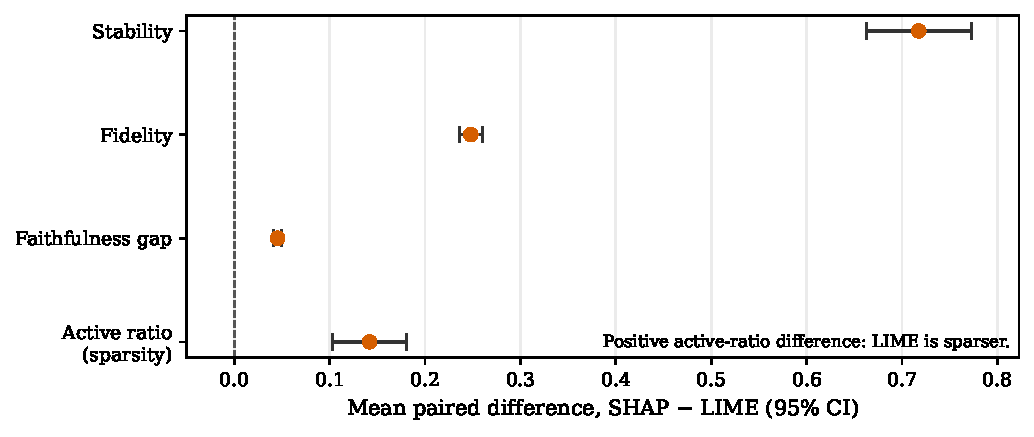
\includegraphics[width=0.8\linewidth]{figures/fig_b1_quality_endpoints.pdf}
\caption{Mean paired difference (SHAP $-$ LIME) with its 95\% confidence
interval for the quality-oriented primary endpoints ($n=75$ matched cells),
as in Table~\ref{tab:paired_main}. For the active ratio, a positive
difference means SHAP is denser, that is, LIME is sparser}
\label{fig:quality_endpoints}
\end{figure}

\subsection{Reproducibility across Seeds}

To characterize how much the readings vary with the seed, the coefficient
of variation (CV\,=\,SD/mean) was computed across the five seeds of the
random-forest stratum at $N=100$ (Table~\ref{tab:cv_reproducibility}); the
medians over all fifteen $(N, \mathrm{model})$ strata are similar ($0.9$,
$1.4$, $2.3$ and $88.2\%$ in the table's row order). SHAP yields highly
reproducible fidelity and stability readings ($\mathrm{CV}<1\%$). LIME
fidelity is acceptable ($\mathrm{CV}=2.6\%$), whereas LIME stability has
$\mathrm{CV}=86.2\%$. That figure mostly reflects the denominator: when the
mean cosine similarity is near zero, any nonzero variation produces an
extreme relative deviation. In absolute terms the spread is small (seed SD
$0.015$): the informative result is the level itself, which is near zero
under the reference configuration.

\begin{table}[htb]
\centering
\caption{Coefficient of variation (CV\,=\,SD/mean) across the five seeds of
the random-forest, $N=100$ stratum for the two primary quality endpoints.
The CV is uninformative for LIME stability, whose mean is near zero}
\label{tab:cv_reproducibility}
\begin{tabular}{lcc}
\toprule
Method -- Metric    & CV & Reproducible? \\
\midrule
SHAP -- Fidelity    & 0.8\%     & Yes \\
SHAP -- Stability   & 0.7\%     & Yes \\
LIME -- Fidelity    & 2.6\%     & Yes \\
LIME -- Stability   & 86.2\%    & CV not meaningful \\
\bottomrule
\end{tabular}
\end{table}

\subsection{Runtime: the Ordering Depends on the Model Family}
\label{sec:runtime}

The cost difference is significant but strongly heterogeneous. SHAP is
slower in 59 of 75 matched cells. The matched-cell median cost is 684.1 ms
for SHAP against 65.7 ms for LIME, and the median per-cell SHAP/LIME cost
ratio is approximately $5.3\times$. The SHAP distribution is heavy-tailed,
so its mean lies far above its median (the per-method means are reported
in~\cite{herrera2026framework}): the 90th and 95th percentile latencies are
approximately 51,456 ms and 67,066 ms, respectively, compared with
12,825 ms and 13,192 ms for LIME. This tail is concentrated in KernelSHAP
contexts, especially the SVM.

The quality ordering (stability, sparsity direction, fidelity, faithfulness
gap) is the same in every model family. The cost ordering is not. SHAP is
faster in all 15 XGBoost matched cells and in one SVM cell, whereas the
logistic regression, random forest and MLP cells are uniformly SHAP-slower
(Figure~\ref{fig:runtime_heterogeneity}, Table~\ref{tab:cost_by_model}).
The two tree ensembles behave in opposite ways. For XGBoost, \texttt{TreeExplainer} was faster than LIME in
all 15 matched cells (median 18.1~ms vs.\ 61.8~ms). For random forests it
was slower in all 15 cells (median 1,262.4~ms vs.\ 335.6~ms). A candidate
explanation, not tested here, is that the cost of \texttt{TreeExplainer}
grows with the number and depth of the trees. For
the non-tree models, where SHAP runs in kernel mode, LIME has the lower
median runtime (53.3~ms vs.\ 694.6~ms). ``LIME is faster'' is therefore a
majority statement in this cohort, not a property of the two methods, and
``SHAP is fast on tree models'' does not hold for tree models in general.

\begin{table}[htb]
\centering
\caption{Median per-instance cost by model group on the matched cells, and
the number of cells in which SHAP was the faster method. SHAP uses
\texttt{TreeExplainer} for the two tree ensembles and
\texttt{KernelExplainer} for the non-tree models}
\label{tab:cost_by_model}
\begin{tabular}{lrrrr}
\toprule
Model group & Cells & SHAP median (ms) & LIME median (ms) & SHAP faster \\
\midrule
XGBoost                             & 15 & 18.1    & 61.8  & 15 of 15 \\
Random forest                       & 15 & 1,262.4 & 335.6 & 0 of 15 \\
Non-tree (logreg, SVM, MLP)         & 45 & 694.6   & 53.3  & 1 of 45 \\
\bottomrule
\end{tabular}
\end{table}

\begin{figure}[htb]
\centering
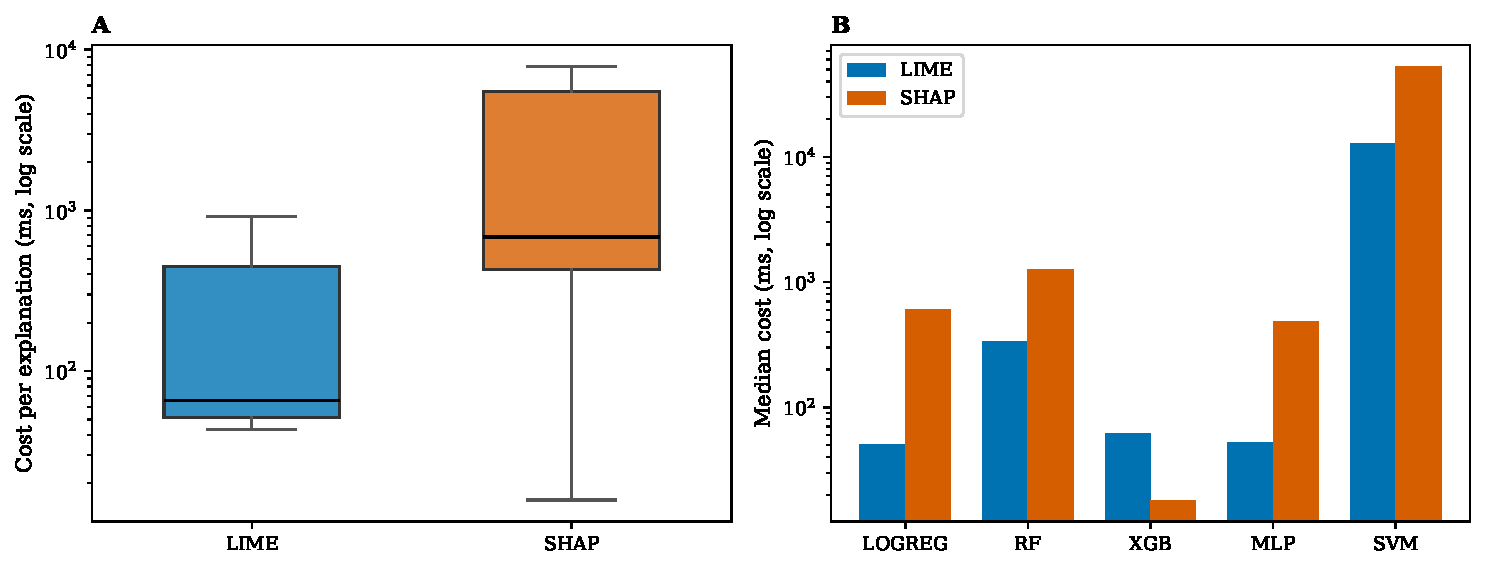
\includegraphics[width=0.85\linewidth]{figures/fig_b2_runtime_heterogeneity.pdf}
\caption{Runtime behavior under matched-cell pairing ($n=75$). (A)
Overall cost distribution by method (log scale). (B) Model-level
median cost (log scale), showing the XGBoost exception where SHAP is
faster while other families are SHAP-slower}
\label{fig:runtime_heterogeneity}
\end{figure}

\subsection{Cross-Dataset Extension}
\label{sec:exp3}

To probe external validity within tabular classification, a cross-dataset
study (EXP3) compared SHAP, LIME and Anchors~\cite{ribeiro2018anchors} on
two further binary classification datasets: Breast Cancer
Wisconsin~\cite{dua2019uci,wolberg1993breast} ($n=569$, 30 continuous
features) and German Credit~\cite{dua2019uci,hofmann1994statlog}
($n=1{,}000$, 20 mixed features). Both used random forest and XGBoost
models across three random seeds each, yielding 12 paired
dataset--model--seed comparisons per method pair.

\textbf{Fidelity ordering (SHAP vs.\ Anchors).} SHAP exceeds Anchors in
fidelity in all 12 paired combinations (Table~\ref{tab:exp3_fidelity}),
with mean gaps ranging from $+0.26$ (German Credit, XGB) to $+0.51$ (Breast
Cancer, RF).

\begin{table}[htb]
\centering
\caption{Cross-dataset extension: mean Anchors fidelity (3-seed average)
and the paired SHAP$-$Anchors fidelity gap. The gap is positive in all 12
paired combinations. SHAP fidelity levels for this cohort are reported
in~\cite{herrera2026framework}; the Anchors levels and the gaps are
contributed here}
\label{tab:exp3_fidelity}
\begin{tabular}{llcc}
\toprule
Dataset        & Model & Anchors & Gap (SHAP $-$ Anchors) \\
\midrule
Breast Cancer  & RF    & 0.265   & $+0.514$ \\
Breast Cancer  & XGB   & 0.208   & $+0.409$ \\
German Credit  & RF    & 0.351   & $+0.363$ \\
German Credit  & XGB   & 0.451   & $+0.260$ \\
\bottomrule
\end{tabular}
\end{table}

\textbf{LIME on the further datasets.} Table~\ref{tab:exp3_lime} reports
LIME fidelity and stability on the same datasets, with the paired
SHAP$-$LIME fidelity gap. Two findings follow.
First, SHAP $>$ LIME fidelity holds on German Credit (mean gaps $+0.23$ for
RF and $+0.24$ for XGB, positive for every seed), in the direction found on
Adult. On Breast Cancer the fidelity gap narrows substantially: SHAP leads
LIME by only $+0.07$ (RF) and $+0.07$ (XGB), compared to $+0.27$ (RF) and
$+0.21$ (XGB) in the corresponding model strata on Adult. Second, LIME
\emph{stability} on these datasets ($0.75$--$0.93$) is an order of
magnitude higher than on Adult, where it is near zero, at the same
reference kernel width. The near-zero stability observed on Adult is
therefore not a fixed property of LIME.

\begin{table}[!htb]
\centering
\caption{Cross-dataset extension: mean fidelity and stability (3-seed
average) for LIME, and the paired SHAP$-$LIME fidelity gap. Stability is
the mean pairwise cosine similarity under $T=15$ Gaussian perturbations
($\sigma=0.1$), the protocol of the main cohort. For comparison, LIME on
Adult in the matched model strata: fidelity $0.457$ (RF) and $0.553$ (XGB);
stability $\approx 0.01$--$0.02$ across all model families}
\label{tab:exp3_lime}
\begin{tabular}{llccccc}
\toprule
Dataset        & Model & Fidelity & Gap (SHAP $-$ LIME) & Stability & Sparsity & Cost (ms) \\
\midrule
Breast Cancer  & RF    & 0.713    & $+0.07$ & 0.922     & 0.331    & 12.3 \\
Breast Cancer  & XGB   & 0.543    & $+0.07$ & 0.927     & 0.331    & 7.5  \\
German Credit  & RF    & 0.483    & $+0.23$ & 0.854     & 0.163    & 21.1 \\
German Credit  & XGB   & 0.468    & $+0.24$ & 0.748     & 0.163    & 10.2 \\
\bottomrule
\end{tabular}
\end{table}

SHAP stability was not instrumented in the cross-dataset study, so a direct
SHAP--LIME stability comparison on Breast Cancer and German Credit is not
available.

\subsection{LIME Stability Depends on the Kernel Width}
\label{sec:kernel}

A probe on Adult varied the LIME kernel width with everything else fixed
(random forest, seed 42, $N=100$, \texttt{num\_samples=1000},
\texttt{num\_features=10}). Table~\ref{tab:kw} reports the result. Fidelity
and stability are computed over the instances that have at least one
non-zero weight. The probe covers one model and one seed, so it shows that
the dependence exists; it does not measure its size across models.

\begin{table}[htb]
\centering
\caption{LIME sensitivity to \texttt{kernel\_width} on Adult (random
forest, seed 42, $N=100$). Reference condition: \texttt{kernel\_width=3.0}}
\label{tab:kw}
\begin{tabular}{lrcccc}
\toprule
\texttt{kernel\_width} & Valid instances & Fidelity & Stability & Sparsity & Cost (ms) \\
\midrule
0.25  & 0/100 (degenerate) & ---   & ---   & 0.000 & 30 \\
0.75  & 0/100 (degenerate) & ---   & ---   & 0.000 & 30 \\
3.0 \emph{(ref.)} & 96/100 & 0.518 & 0.000 & 0.087 & 30 \\
10.0  & 100/100            & 0.441 & 0.664 & 0.093 & 32 \\
\bottomrule
\end{tabular}
\end{table}

Kernel widths of 0.25 and 0.75 produce zero-weight explanations for all 100
instances, because the exponential neighborhood collapses in the
103-dimensional one-hot-encoded space. The reference width of 3.0 is the
smallest of the tested settings that yields usable explanations. Widening
the kernel to $10.0$ raises stability to $0.664$ at a cost in fidelity
($0.518 \rightarrow 0.441$). Together with the cross-dataset result, where
LIME reaches $0.75$--$0.93$ at the reference width, the probe supports a
bounded conclusion: under the reference kernel width, LIME's stability on
Adult is near zero; it rises with the kernel width and is high on two
lower-dimensional datasets, so it is modulated by the configuration and by
the feature space. Adult's one-hot encoding is a candidate cause, and the
stability protocol itself may contribute: the Gaussian noise is added to
every transformed feature, including the one-hot indicator columns, which
then take values that no real instance has. Breast Cancer has no
categorical feature. No experiment here separates the encoding from the
perturbation scheme, and the two further datasets also differ from Adult in
size, class balance and the mix of continuous and categorical features, so
this design does not isolate either cause. The near-zero reading should not be taken as a
configuration-independent property of LIME.

\subsection{Sensitivity of the Fidelity Ordering to the Masking Scheme}
\label{sec:masking}

The fidelity and faithfulness-gap metrics mask features independently.
Adult contains associated features, so a masked instance may fall outside
the training distribution, where model outputs are less reliable. To assess
whether this changes the method ordering, a probe reused the stored top-10
explanations of the five Adult random-forest runs at $N=50$, one per seed,
and recomputed the prediction-drop metrics under four masking schemes:
independent zero masking, mean replacement, marginal empirical replacement,
and grouped mean replacement, which masks associated feature sets together
(for example \texttt{education} and \texttt{education-num}).
Table~\ref{tab:masking} reports the result.

\begin{table}[htb]
\centering
\caption{SHAP--LIME top-$k$ prediction-drop advantage and drop-correlation
advantage under four masking schemes (Adult random-forest stratum, five
runs at $N=50$, one per seed). The SHAP direction is positive in all five
paired seed cells under every scheme}
\label{tab:masking}
\begin{tabular}{lcc}
\toprule
Masking scheme & Mean SHAP--LIME gap & Mean drop-correlation delta \\
\midrule
Independent zero masking      & +0.098 & +0.515 \\
Mean replacement               & +0.098 & +0.512 \\
Marginal empirical replacement & +0.081 & +0.625 \\
Grouped mean replacement       & +0.053 & +0.494 \\
\bottomrule
\end{tabular}
\end{table}

SHAP's advantage is positive in all five paired cells under every scheme.
Its magnitude, measured as the prediction-drop gap, does not increase, and
falls overall, as the masking takes more of the feature dependence into
account ($+0.098 \rightarrow +0.098 \rightarrow +0.081 \rightarrow
+0.053$). The drop-correlation delta does not follow this ordering: it is
highest under marginal empirical replacement ($+0.625$) and lowest under
grouped mean replacement ($+0.494$). With five pairs, the exact Wilcoxon
test cannot reach $\alpha = 0.05$ under any scheme, so this agreement is
descriptive. The probe uses stored top-10 explanations, not full
attribution vectors, and is a stress test of the construct, not a
replacement for the primary analysis: the direction holds in every pair,
and the magnitude depends in part on the masking protocol.

% -----------------------------------------------------------------------
\section{Discussion}
\label{sec:discussion}
% -----------------------------------------------------------------------

\subsection{What the Paired Analysis Adds}

The four hypotheses are supported on Adult: SHAP is more stable (RQ1) and
scores higher on fidelity and faithfulness gap (RQ4); LIME is sparser as
configured (RQ2) and cheaper in most cells (RQ3). The analysis on the full
grid confirms the direction that the earlier 45-cell test found, extends it
to the SVM and the MLP, and attaches an interval and an effect size to each
endpoint; the fidelity and stability differences have the same sign in
every cell.
SHAP delivers higher stability and fidelity at a substantially higher
expected runtime; LIME delivers lower latency and more compact explanations
at the cost of robustness.

Two of these results come with conditions, and the conditions are the part
most likely to matter in practice. The runtime result (RQ3) reverses
between XGBoost and random forests, two models that a guideline would group
together as ``tree-based''. The stability result (RQ1) is measured at one
LIME kernel width on one feature space; a wider kernel or a
lower-dimensional dataset raises LIME's stability from near zero to between
$0.664$ and $0.927$. A comparison run on one dataset with one
configuration would report either of these as a property of the methods.

One candidate reason for SHAP's fidelity advantage is that SHAP ties
attribution mass to the model's response to feature removal: local accuracy
means the attributions sum to the prediction change relative to the
background distribution~\cite{lundberg2017unified}, and removal-based
fidelity asks a related question. This mechanism was not tested and carries
no guarantee: the masking used here replaces features with reference values
and not with SHAP's background expectation, KernelSHAP is itself a sampled
estimate, and the advantage is small on Breast Cancer.

\subsection{Recommendation Conditioned on the Model Architecture}
\label{sec:recommendations}

Table~\ref{tab:hybrid_deployment} states the recommendation in two tiers.
The first-tier criterion is not a preference for a method. It is a function
of the model architecture: where a model-aware explainer is also fast, as
\texttt{TreeExplainer} was for XGBoost, the trade-off between fidelity and
latency disappears and SHAP is the better choice in both tiers; where it is
not, as for the random forests here, the trade-off remains and has to be
measured for the deployed model.

\begin{table}[htb]
\centering
\caption{Recommendation by deployment tier, conditioned on the model
architecture}
\label{tab:hybrid_deployment}
\begin{tabularx}{\linewidth}{p{2.4cm} >{\raggedright\arraybackslash}p{4.2cm} X}
\toprule
\textbf{Tier} & \textbf{Recommendation} & \textbf{Evidence and condition} \\
\midrule
Tier 1: real-time, end-user facing &
\textbf{SHAP} (\texttt{TreeExplainer}) for XGBoost; \textbf{LIME} for
models without a fast model-aware explainer; for other tree ensembles,
measure latency before choosing. &
For XGBoost, SHAP was faster in all 15 matched cells and more faithful.
For random forests it was slower in all 15 cells. For non-tree models LIME
has the lower median runtime (Section~\ref{sec:runtime}). Applies when
sub-second latency and compact explanations matter more than maximum
fidelity. \\[4pt]
Tier 2: auditing, model analysis &
\textbf{SHAP.} &
Consistent paired advantages in stability, fidelity and faithfulness gap
($d_z = 3.00$, $4.82$, $2.63$). Applies to offline or analyst-mediated work
that tolerates latencies of seconds to minutes; the sample budget depends
on whether SHAP runs in tree-specific or kernel mode. \\
\bottomrule
\end{tabularx}
\end{table}

\subsection{Validity and Limitations}
\label{sec:validity}

\textbf{Ranking claims, not validity claims.} The differences reported here
are comparative performance within a benchmark protocol. A claim that an
explanation is correct for a task would need stronger evidence: ground
truth from synthetic or transparent models, perturbation protocols that
respect feature dependence, or human-centered
validation~\cite{haufe2026formalization,doshivelez2017rigorous}. Formal
analyses show that several attribution families assign high importance to
suppressor variables when features are
dependent~\cite{wilming2022scrutinizing,wilming2023theoretical}, and
faithfulness-style evaluations are informative but do not settle
correctness on their own~\cite{jacovi2020faithfulness,rong2022consistent}.

\textbf{Configuration.} Both methods were run with one fixed reference
configuration. The cost gap reflects the method family and the concrete
implementation pathway (tree-specific or kernel SHAP). The kernel-width
probe covers one model and one seed. Sensitivity to the SHAP background
sample and to the kernel width in other models was not examined.

\textbf{Execution hosts and the cost endpoint.} Cost is per-instance
wall-clock time, and the runs were executed on several workstations whose
processor and memory specifications were not recorded
(Section~\ref{sec:infrastructure}). The two members of a paired cell are
matched on model, seed and $N$, but did not necessarily run on the same
host. Absolute latencies, and the medians reported here, include
between-host variance and are indicative of this environment; they are not
hardware-normalized measurements. The quality endpoints do not depend on
the host.

\textbf{Generalization.} Table~\ref{tab:generalizability_boundary} states
the boundary of each claim. The comparison is limited to tabular binary
classification; image, text, graph and time-series explanations need
different masking schemes and endpoints and were not tested. The endpoints
measure how well an explanation tracks the model it explains. They say
nothing about whether that model is accurate or fair, and nothing about
whether a person decides better with the explanation.

\begin{table}[htb]
\centering
\caption{Generalizability boundary of the empirical claims}
\label{tab:generalizability_boundary}
\begin{tabularx}{\linewidth}{p{3.0cm} X X}
\toprule
\textbf{Claim} & \textbf{Evidence} & \textbf{Generalization status} \\
\midrule
SHAP $>$ LIME stability & Adult matched cells, one LIME kernel width & Holds for the Adult protocol only; LIME stability is high on two further datasets, where SHAP stability was not measured \\
SHAP $>$ LIME fidelity & Adult, plus German Credit and Breast Cancer & Supported within tabular classification, with a small gap on Breast Cancer; not established for other data types \\
LIME lower runtime & Adult, model-dependent & Bounded by the model architecture and the SHAP implementation; \texttt{TreeExplainer} reverses the ordering for XGBoost but not for random forests \\
SHAP $>$ Anchors fidelity & Breast Cancer and German Credit & Fidelity ordering only; not a stability or runtime result \\
Usefulness for people & No participant study & Not established \\
\bottomrule
\end{tabularx}
\end{table}

% -----------------------------------------------------------------------
\section{Conclusions}
\label{sec:conclusion}
% -----------------------------------------------------------------------

On 75 matched cells of the Adult dataset, SHAP shows consistent paired
advantages over LIME in stability ($d_z = 3.00$), fidelity ($d_z = 4.82$)
and faithfulness gap ($d_z = 2.63$), and LIME produces sparser explanations
and runs faster in most model contexts. A cross-dataset extension supports
the fidelity direction on two further tabular datasets.

The choice between the two methods is a matter of fit for purpose, and two
of the usual rules of thumb need a condition. SHAP is not fast on tree
models in general: it was faster than LIME for XGBoost and slower for
random forests. LIME is not unstable in general: its near-zero stability on
Adult is specific to the reference kernel width and to that feature space.
The practical recommendation is to prefer SHAP where stability and fidelity
dominate, to prefer LIME where latency dominates and no fast model-aware
explainer exists, and to measure latency for the deployed model before
relying on either rule.

Future work should instrument SHAP stability on further datasets, vary the
SHAP background sample and the LIME kernel width across models, and extend
the comparison beyond tabular classification. Whether either method helps
people decide is a separate question that needs a study with participants.

\ifblind\else
\section*{Acknowledgments}

The author thanks Miguel Herrero Uceda, PhD, for his revision of this
manuscript and for his constructive comments during its development.
\fi

\section*{Data and Code Availability}
\label{sec:artifacts}

The experimental code, the run artifacts and the analysis exports are
available in \ifblind a public repository and in a versioned archive with a
DOI, both released under the MIT License; their addresses are withheld for
double-blind review\else the public repository
\url{https://github.com/jonnabio/xai-eval-framework}, released under the
MIT License, and in its archived release, \zenodoversiondoi{}\fi. The
artifacts needed to reproduce this study are the main-cohort results
(\path{experiments/exp2_scaled/results/}), the inferential exports
(\path{outputs/analysis/paper_a_exp2_stats/}), the cross-dataset results
(\path{experiments/exp3_cross_dataset/results/} and
\path{outputs/analysis/exp3_lime_results.csv}), the kernel-width probe
(\path{outputs/analysis/lime_kernel_width_sensitivity.csv}) and the
masking-sensitivity exports
(\path{outputs/analysis/exp6_masking_sensitivity/}). Every reported value
is re-derived from these files by a verification script that runs in
continuous integration.

\begin{thebibliography}{99}

\bibitem{ribeiro2016why}
M.~T. Ribeiro, S. Singh, and C. Guestrin, ``Why should I trust you?:
Explaining the predictions of any classifier,'' in \emph{Proc. 22nd ACM
SIGKDD Int. Conf. Knowledge Discovery and Data Mining}, 2016,
pp.~1135--1144. [Online]. Available:
\url{https://doi.org/10.1145/2939672.2939778}

\bibitem{lundberg2017unified}
S.~M. Lundberg and S.-I. Lee, ``A unified approach to interpreting model
predictions,'' in \emph{Advances in Neural Information Processing Systems},
2017, pp.~4765--4774.

\bibitem{retzlaff2024posthoc}
C.~O. Retzlaff, A. Angerschmid, A. Saranti, D. Schneeberger, R. R\"{o}ttger,
H. M\"{u}ller, and A. Holzinger, ``Post-hoc vs ante-hoc explanations: xAI
design guidelines for data scientists,'' \emph{Cognitive Systems Research},
vol.~86, p.~101243, 2024. [Online]. Available:
\url{https://doi.org/10.1016/j.cogsys.2024.101243}

\bibitem{ali2023trustworthy}
S. Ali, T. Abuhmed, S. El-Sappagh, K. Muhammad, J.~M. Alonso-Moral,
R. Confalonieri, R. Guidotti, J. Del~Ser, N. D\'{i}az-Rodr\'{i}guez, and
F. Herrera, ``Explainable Artificial Intelligence (XAI): What we know and
what is left to attain Trustworthy Artificial Intelligence,''
\emph{Information Fusion}, vol.~99, p.~101805, 2023. [Online]. Available:
\url{https://doi.org/10.1016/j.inffus.2023.101805}

\bibitem{nauta2023anecdotal}
M. Nauta, J. Trienes, S. Pathak, E. Nguyen, M. Peters, Y. Schmitt,
J. Schl\"{o}tterer, M. van Keulen, and C. Seifert, ``From anecdotal evidence
to quantitative evaluation methods: A systematic review on evaluating
explainability,'' \emph{ACM Computing Surveys}, vol.~55, no.~13s,
pp.~1--42, 2023. [Online]. Available:
\url{https://doi.org/10.1145/3583558}

\bibitem{canha2025benchmark}
D. Canha, S. Kubler, K. Fr\"{a}mling, and G. Fagherazzi, ``A
functionally-grounded benchmark framework for XAI methods: Insights and
foundations from a systematic literature review,'' \emph{ACM Computing
Surveys}, vol.~57, no.~12, pp.~1--40, 2025. [Online]. Available:
\url{https://doi.org/10.1145/3737445}

\bibitem{longo2024manifesto}
L. Longo, M. Brcic, F. Cabitza, J. Choi, R. Confalonieri, J. Del~Ser,
R. Guidotti, Y. Hayashi, F. Herrera, A. Holzinger, R. Jiang, H. Khosravi,
F. Lecue, G. Malgieri, A. P\'{a}ez, W. Samek, J. Schneider, T. Speith, and
S. Stumpf, ``Explainable artificial intelligence (XAI) 2.0: A manifesto of
open challenges and interdisciplinary research directions,''
\emph{Information Fusion}, vol.~106, p.~102301, 2024. [Online]. Available:
\url{https://doi.org/10.1016/j.inffus.2024.102301}

\bibitem{pawlicki2024metrics}
M. Pawlicki, A. Pawlicka, F. Uccello, S. Szelest, S. D'Antonio, R. Kozik,
and M. Chora\'{s}, ``Evaluating the necessity of the multiple metrics for
assessing explainable AI: A critical examination,'' \emph{Neurocomputing},
vol.~602, p.~128282, 2024. [Online]. Available:
\url{https://doi.org/10.1016/j.neucom.2024.128282}

\bibitem{zheng2025ffidelity}
X. Zheng, F. Shirani, Z. Chen, C. Lin, W. Cheng, W. Guo, and D. Luo,
``F-Fidelity: A robust framework for faithfulness evaluation of explainable
AI,'' in \emph{13th Int. Conf. Learning Representations (ICLR)}, 2025.
[Online]. Available: \url{https://openreview.net/forum?id=X0r4BN50Dv}

\bibitem{herrera2026framework}
J. Herrera-V\'asquez and M. Herrero-Uceda, ``A framework for rigorous
evaluation of model-agnostic explainability methods: multi-metric
statistical benchmarking, operational protocol, and reproducibility,''
\emph{Revista de Investigaci\'on Multidisciplinaria Iberoamericana (RIMI)},
no.~3, 2026. [Online]. Available:
\url{https://doi.org/10.69850/rimi.vi3.307}

\bibitem{bhatt2020evaluating}
U. Bhatt, A. Weller, and J.~M.~F. Moura, ``Evaluating and aggregating
feature-based model explanations,'' in \emph{Proc. 29th Int. Joint Conf.
Artificial Intelligence (IJCAI)}, 2020, pp.~3016--3022. [Online]. Available:
\url{https://doi.org/10.24963/ijcai.2020/417}

\bibitem{samek2017evaluating}
W. Samek, A. Binder, G. Montavon, S. Lapuschkin, and K.-R. M\"{u}ller,
``Evaluating the visualization of what a deep neural network has learned,''
\emph{IEEE Trans. Neural Networks and Learning Systems}, vol.~28, no.~11,
pp.~2660--2673, 2017. [Online]. Available:
\url{https://doi.org/10.1109/TNNLS.2016.2599820}

\bibitem{hooker2019benchmark}
S. Hooker, D. Erhan, P.-J. Kindermans, and B. Kim, ``A benchmark for
interpretability methods in deep neural networks,'' in \emph{Advances in
Neural Information Processing Systems}, vol.~32, 2019, pp.~9737--9748.

\bibitem{alvarezmelis2018robustness}
D. Alvarez-Melis and T.~S. Jaakkola, ``On the robustness of
interpretability methods,'' in \emph{ICML Workshop on Human
Interpretability in Machine Learning (WHI 2018)}, 2018. [Online].
Available: \url{https://arxiv.org/abs/1806.08049}

\bibitem{hedstrom2023quantus}
A. Hedstrom, L. Weber, D. Bareeva, D. Krakowczyk, F. Motzkus, W. Samek,
S. Lapuschkin, and M.~M.-C. Hohne, ``Quantus: An explainable AI toolkit for
responsible evaluation of neural network explanations and beyond,''
\emph{Journal of Machine Learning Research}, vol.~24, pp.~1--11, 2023. [Online]. Available:
\url{https://jmlr.org/papers/v24/22-0142.html}

\bibitem{agarwal2022openxai}
C. Agarwal, D. Ley, S. Krishna, E. Saxena, M. Pawelczyk, N. Johnson,
I. Puri, M. Zitnik, and H. Lakkaraju, ``OpenXAI: Towards a transparent
evaluation of model explanations,'' in \emph{36th Conf. Neural Information
Processing Systems, Datasets and Benchmarks Track}, 2022. [Online].
Available: \url{https://openreview.net/forum?id=MU2495w47rz}

\bibitem{adebayo2018sanity}
J. Adebayo, J. Gilmer, M. Muelly, I. Goodfellow, M. Hardt, and B. Kim,
``Sanity checks for saliency maps,'' in \emph{Advances in Neural
Information Processing Systems}, vol.~31, 2018, pp.~9525--9536.

\bibitem{rong2022consistent}
Y. Rong, T. Leemann, V. Borisov, G. Kasneci, and E. Kasneci, ``A consistent
and efficient evaluation strategy for attribution methods,'' in \emph{Proc.
39th Int. Conf. Machine Learning}, 2022, pp.~18770--18795. [Online]. Available:
\url{https://proceedings.mlr.press/v162/rong22a.html}

\bibitem{slack2020fooling}
D. Slack, S. Hilgard, E. Jia, S. Singh, and H. Lakkaraju, ``Fooling LIME
and SHAP: Adversarial attacks on post hoc explanation methods,'' in
\emph{Proc. AAAI/ACM Conf. AI, Ethics, and Society}, 2020, pp.~180--186.
[Online]. Available: \url{https://doi.org/10.1145/3375627.3375830}

\bibitem{kumar2020problems}
I.~E. Kumar, S. Venkatasubramanian, C. Scheidegger, and S.~A. Friedler,
``Problems with Shapley-value-based explanations as feature importance
measures,'' in \emph{Proc. 37th Int. Conf. Machine Learning}, 2020,
pp.~5491--5500. [Online]. Available: \url{https://arxiv.org/abs/2002.11097}

\bibitem{kohavi1996scaling}
R. Kohavi, ``Scaling up the accuracy of Naive-Bayes classifiers: A
decision-tree hybrid,'' in \emph{Proc. 2nd Int. Conf. Knowledge Discovery
and Data Mining}, 1996, pp.~202--207.

\bibitem{becker1996adult}
B. Becker and R. Kohavi, ``Adult [dataset],'' UCI Machine Learning
Repository, 1996. [Online]. Available:
\url{https://doi.org/10.24432/C5XW20}

\bibitem{breiman2001random}
L. Breiman, ``Random forests,'' \emph{Machine Learning}, vol.~45, no.~1,
pp.~5--32, 2001. [Online]. Available:
\url{https://doi.org/10.1023/A:1010933404324}

\bibitem{chen2016xgboost}
T. Chen and C. Guestrin, ``XGBoost: A scalable tree boosting system,'' in
\emph{Proc. 22nd ACM SIGKDD Int. Conf. Knowledge Discovery and Data
Mining}, 2016, pp.~785--794. [Online]. Available:
\url{https://doi.org/10.1145/2939672.2939785}

\bibitem{demsar2006statistical}
J. Dem\v{s}ar, ``Statistical comparisons of classifiers over multiple data
sets,'' \emph{Journal of Machine Learning Research}, vol.~7, pp.~1--30,
2006. [Online]. Available:
\url{https://jmlr.org/papers/v7/demsar06a.html}

\bibitem{wilcoxon1945individual}
F. Wilcoxon, ``Individual comparisons by ranking methods,''
\emph{Biometrics Bulletin}, vol.~1, no.~6, pp.~80--83, 1945. [Online]. Available:
\url{https://doi.org/10.2307/3001968}

\bibitem{lakens2013calculating}
D. Lakens, ``Calculating and reporting effect sizes to facilitate
cumulative science: A practical primer for $t$-tests and ANOVAs,''
\emph{Frontiers in Psychology}, vol.~4, p.~863, 2013. [Online]. Available:
\url{https://doi.org/10.3389/fpsyg.2013.00863}

\bibitem{holm1979simple}
S. Holm, ``A simple sequentially rejective multiple test procedure,''
\emph{Scandinavian Journal of Statistics}, vol.~6, no.~2, pp.~65--70, 1979.

\bibitem{ribeiro2018anchors}
M.~T. Ribeiro, S. Singh, and C. Guestrin, ``Anchors: High-precision
model-agnostic explanations,'' in \emph{Proc. 32nd AAAI Conf. Artificial
Intelligence}, 2018, pp.~1527--1535. [Online]. Available:
\url{https://doi.org/10.1609/aaai.v32i1.11491}

\bibitem{mothilal2020dice}
R.~K. Mothilal, A. Sharma, and C. Tan, ``Explaining machine learning
classifiers through diverse counterfactual explanations,'' in \emph{Proc.
2020 Conf. Fairness, Accountability, and Transparency}, 2020, pp.~607--617. [Online]. Available:
\url{https://doi.org/10.1145/3351095.3372850}

\bibitem{dua2019uci}
D. Dua and C. Graff, ``UCI Machine Learning Repository,'' University of
California, Irvine, School of Information and Computer Science, 2019.
[Online]. Available: \url{http://archive.ics.uci.edu/ml}

\bibitem{wolberg1993breast}
W. Wolberg, O. Mangasarian, N. Street, and W. Street, ``Breast cancer
Wisconsin (diagnostic) [dataset],'' UCI Machine Learning Repository, 1993.
[Online]. Available: \url{https://doi.org/10.24432/C5DW2B}

\bibitem{hofmann1994statlog}
H. Hofmann, ``Statlog (German credit data) [dataset],'' UCI Machine
Learning Repository, 1994. [Online]. Available:
\url{https://doi.org/10.24432/C5NC77}

\bibitem{haufe2026formalization}
S. Haufe, R. Wilming, B. Clark, R. Zhumagambetov, A. Boubekki, J. Martin,
and D. Panknin, ``Explainable AI needs formalization,'' \emph{npj
Artificial Intelligence}, vol.~2, p.~42, 2026. [Online]. Available:
\url{https://doi.org/10.1038/s44387-026-00095-1}

\bibitem{doshivelez2017rigorous}
F. Doshi-Velez and B. Kim, ``Towards a rigorous science of interpretable
machine learning,'' arXiv preprint arXiv:1702.08608, 2017. [Online].
Available: \url{https://arxiv.org/abs/1702.08608}

\bibitem{wilming2022scrutinizing}
R. Wilming, C. Budding, K.-R. M\"{u}ller, and S. Haufe, ``Scrutinizing XAI
using linear ground-truth data with suppressor variables,'' \emph{Machine
Learning}, vol.~111, no.~5, pp.~1903--1923, 2022. [Online]. Available:
\url{https://doi.org/10.1007/s10994-022-06167-y}

\bibitem{wilming2023theoretical}
R. Wilming, L. Kieslich, B. Clark, and S. Haufe, ``Theoretical behavior of
XAI methods in the presence of suppressor variables,'' in \emph{Proc. 40th
Int. Conf. Machine Learning}, vol.~202, 2023, pp.~37091--37107. [Online]. Available:
\url{https://proceedings.mlr.press/v202/wilming23a.html}

\bibitem{jacovi2020faithfulness}
A. Jacovi and Y. Goldberg, ``Towards faithfully interpretable NLP systems:
How should we define and evaluate faithfulness?'' in \emph{Proc. 58th
Annual Meeting of the Association for Computational Linguistics}, 2020,
pp.~4198--4205. [Online]. Available:
\url{https://doi.org/10.18653/v1/2020.acl-main.386}

\end{thebibliography}

\end{document}
